\documentclass{article}%
\usepackage[T1]{fontenc}%
\usepackage[utf8]{inputenc}%
\usepackage{lmodern}%
\usepackage{textcomp}%
\usepackage{lastpage}%
\usepackage[head=40pt,margin=0.5in,bottom=0.6in]{geometry}%
\usepackage{graphicx}%
%
\title{\textbf{Pacientes renales de Táchira sufren la falta de insumos}}%
\author{El Nacional Web}%
\date{06/10/2018}%
%
\begin{document}%
\normalsize%
\maketitle%
\textbf{URL: }%
http://www.el{-}nacional.com/noticias/salud/pacientes{-}renales{-}tachira{-}sufren{-}falta{-}insumos\_254632\newline%
%
\textbf{Periodico: }%
EN, %
ID: %
254632, %
Seccion: %
Salud\newline%
%
\textbf{Palabras Claves: }%
Salud, Táchira, Crisis humanitaria\newline%
%
\textbf{Derecho: }%
2.1%
, Otros Derechos: %
NO\_TIENE%
, Sub Derechos: %
2.1.1%
\newline%
%
\textbf{EP: }%
NO\newline%
\newline%
%
\textbf{\textit{En la unidad de diálisis de barrio Obrero solo funciona siete de las 16 máquinas para dializar~}}%
\newline%
\newline%
%
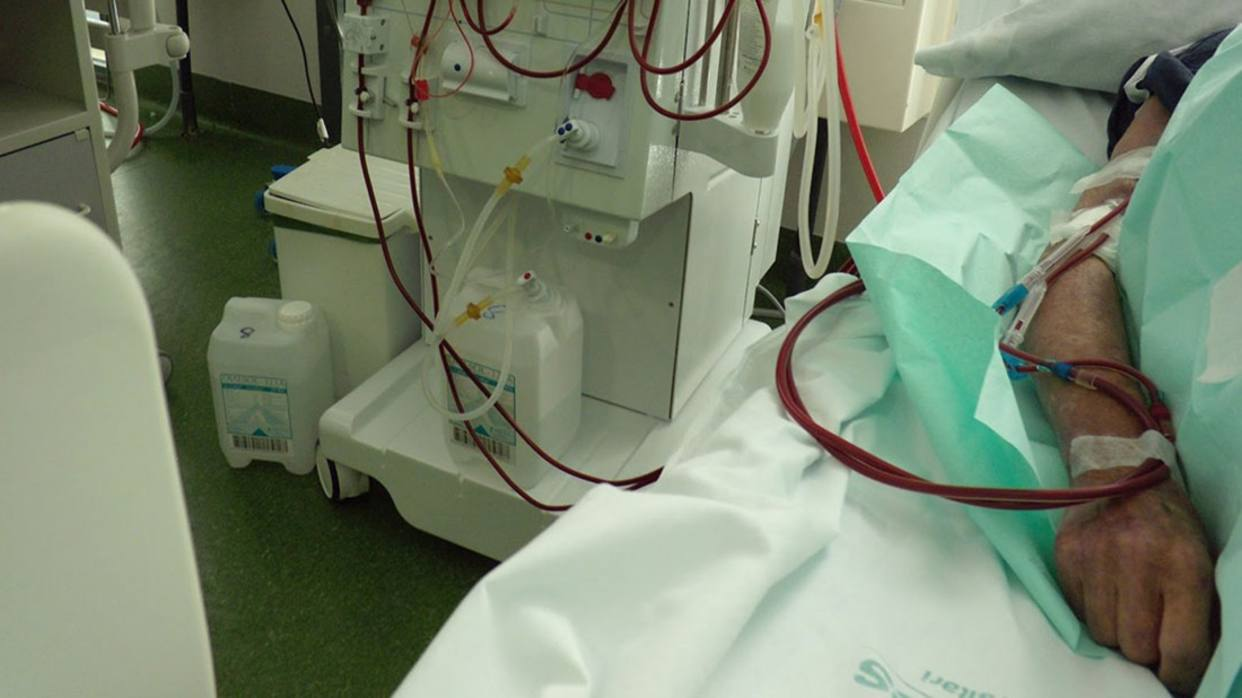
\includegraphics[width=300px]{230.jpg}%
\newline%
%
Los pacientes con tratamiento de hemodiálisis enfrentan cada día la escasez de insumos y la falta de los equipos necesarios para realizarse los procedimientos médicos.%
\newline%
%
Las personas deben reducir la cantidad de diálisis que se hacen a la semana y pasan de 12 sesiones a seis, reseñó~La Nación~de Táchira.%
\newline%
%
En la unidad de diálisis Diasanca, ubicada en~Barrio Obrero solo funcionan siete de las 16 que hay en la unidad.%
\newline%
%
“A través de estas máquinas los pacientes eliminan los líquidos, toxinas, y desde hace más de un mes más de la mitad están inoperativas y entonces para tratar de atenderos a todos se le das dos hoy y media de tratamiento a cada paciente cuando lo normal son tres~horas y media” dijo una enfermera.%
\newline%
%
Hernán Rodríguez, paciente que requiere diálisis, resaltó que no cuentan con insumos y pidió a Coriana Lugo, jefe de Nefrología del Seguro Social en Caracas, que resuelva el problema de las unidades de diálisis del estado Táchira. “El presupuesto asignados para todas las unidades del estado no alcanza ni para una reparación de una máquina” aseguró Rodríguez.%
\newline%
%
Leer más en~La Nación%
\newline%
%
\end{document}